

%%%%%%%%%%%%%%%%%%%%%%%%%%%%%%%%%%% ViennaCL %%%%%%%%%%%%%%%%%%%%%%%%%%%%%%%%%%%%

\begin{frame}{About ViennaCL}

  \begin{block}{About}
   \begin{itemize}
    \item High-level linear algebra C++ library
    \item OpenMP, OpenCL, and CUDA backends
    \item Header-only
    \item Multi-platform
   \end{itemize}
  \end{block}

  \vspace*{-2.3cm}
  \begin{flushright}
   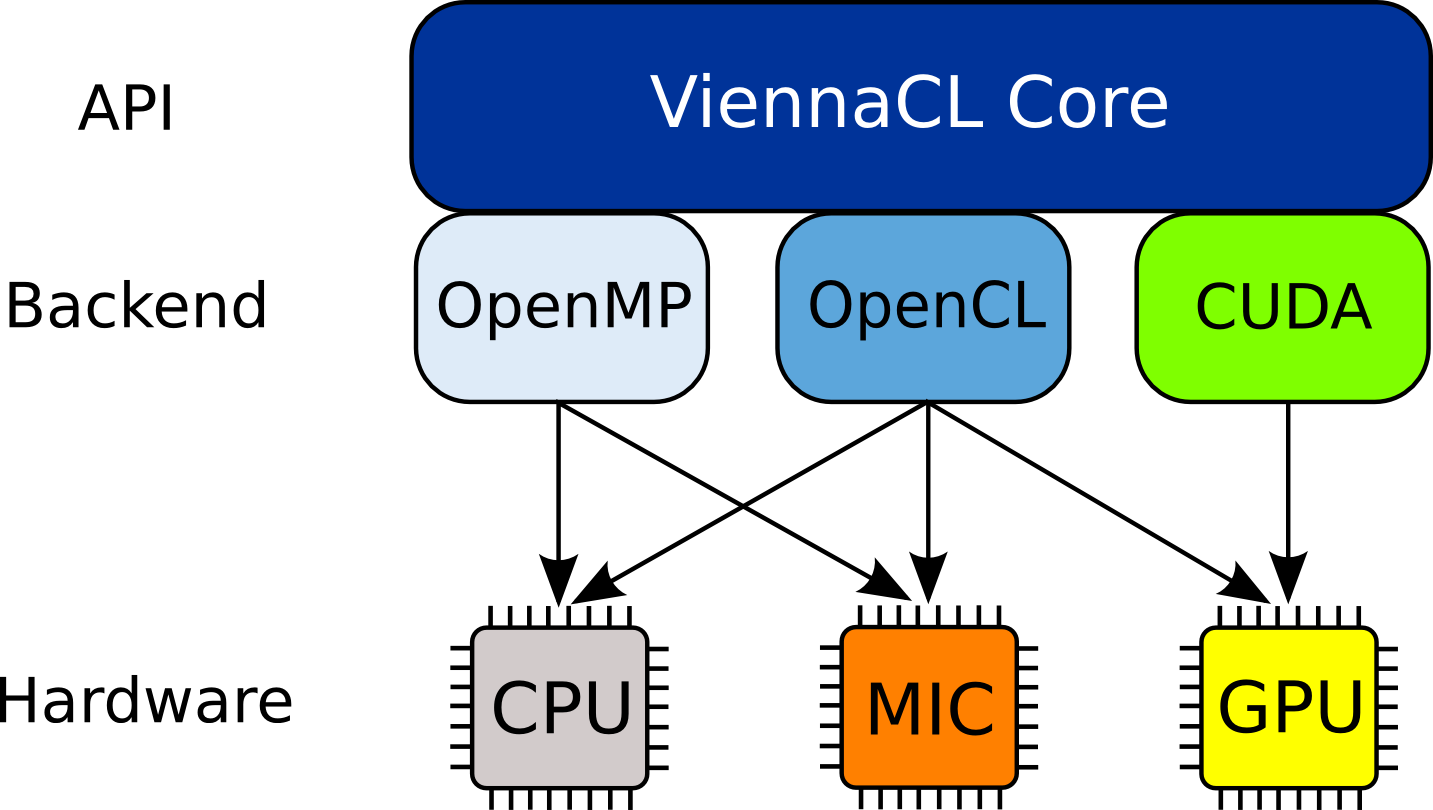
\includegraphics[width=0.4\textwidth]{figures/ViennaCL-arch.png}
  \end{flushright}

  \vspace*{-0.7cm}
  \begin{block}{Dissemination}
    \begin{itemize}
     \item Free Open-Source MIT (X11) License
     \item http://viennacl.sourceforge.net/
     \item 50-100 downloads per week
    \end{itemize}   
  \end{block}

  \begin{block}{Design Rules}
   \begin{itemize}
    \item Reasonable default values
    \item Compatible to Boost.uBLAS whenever possible 
    \item In doubt: clean design over performance
   \end{itemize}
  \end{block}

\end{frame}

%%%%%%%%


%%%%%%%%%%%%%%% Explain ViennaCL types here %%%%%%%%%%%%%%%%%%%%%%

\begin{frame}[fragile]
\frametitle{About ViennaCL}

 \begin{block}{Basic Types}
   \begin{itemize}
    \item scalar
    \item vector
    \item matrix, compressed\_matrix, coordinate\_matrix, ell\_matrix, hyb\_matrix
   \end{itemize}
 \end{block}

 \begin{block}{Data Initialization}
    \begin{itemize}
     \item Using viennacl::copy() 
    \item  { \black
  \begin{lstlisting}
     std::vector<double>      std_x(100);
   ublas::vector<double>    ublas_x(100);
viennacl::vector<double>      vcl_x(100);


for (size_t i=0; i<100; ++i){
    std_x[i] = rand();
  ublas_x[i] = rand();
    vcl_x[i] = rand();  //possible, inefficient
}
  \end{lstlisting} }

%   \item Reuse of C++ STL coding conventions
 \end{itemize}

 \end{block}
\end{frame}



\begin{frame}[fragile]
\frametitle{About ViennaCL}

 \begin{block}{Basic Types}
   \begin{itemize}
    \item scalar
    \item vector
    \item matrix, compressed\_matrix, coordinate\_matrix, ell\_matrix, hyb\_matrix
   \end{itemize}
 \end{block}

 \begin{block}{Data Initialization}
    \begin{itemize}
     \item Using viennacl::copy() 
    \item  { \black
  \begin{lstlisting}
     std::vector<double>      std_x(100);
   ublas::vector<double>    ublas_x(100);
viennacl::vector<double>      vcl_x(100);

/* setup of std_x and ublas_x omitted */

viennacl::copy(std_x.begin(), std_x.end(),
               vcl_x.begin());   //to GPU
viennacl::copy(vcl_x.begin(), vcl_x.end(),
               ublas_x.begin()); //to CPU
  \end{lstlisting} }

%   \item Reuse of C++ STL coding conventions
 \end{itemize}

 \end{block}
\end{frame}


\begin{frame}[fragile]
\frametitle{About ViennaCL}

 \begin{block}{Basic Types}
   \begin{itemize}
    \item scalar
    \item vector
    \item matrix, compressed\_matrix, coordinate\_matrix, ell\_matrix, hyb\_matrix
   \end{itemize}
 \end{block}

 \begin{block}{Data Initialization}
    \begin{itemize}
     \item Using viennacl::copy() 
    \item  { \black
  \begin{lstlisting}
     std::vector<std::vector<double> >    std_A;
   ublas::matrix<double>                ublas_A;
viennacl::matrix<double>                  vcl_A;

/* setup of std_A and ublas_A omitted */

viennacl::copy(std_A,
               vcl_A);    // CPU to GPU
viennacl::copy(vcl_A,
               ublas_A);  // GPU to CPU
  \end{lstlisting} }
 \end{itemize}

 \end{block}
\end{frame}


